
%  \section{The PSF profile analysis}

Since the 6-parameter PSF fits was adopted by the SDSS processing
pipeline, significant progress has been made in validating the von
Karman model of the atmosphere and measuring the associated outer
scale. See, for example, \cite{Tokovinin2002},
\cite{Boccas2004}, and \cite{MartinezMessenger}.
In this section, we describe our 2-parameter fits to the SDSS PSF
profiles using the von Karman atmosphere model.

Our fits to each PSF profile is a 2-step process. First we fit the
measured PSF profile to a von Karman PSF, with only one free parameter -
the FWHM of the von Karman profile. Although the fitted
curve agrees with the input data points very well, better than the
original 6-parameter double-Gaussian fit in general, it doesn't always describe
the PSF tail beyond $\sim 15$ arcsec radius. This is obvious, because
it is known that the PSF tails in the optical bands can be quite
different due to the properties of the CCDs.
For example, the $i$-band PSF has ``stronger tails''
because of scattering in the CCD.  The Si is transparent at long $i$-band wavelengths 
so light goes all the way through the chip and is reflected off the solder, and passes 
back up through the Si. This effect is not visible in the $z$-band because in this case
thick front-side chips are used (in all other bands, thin back-side chips are used). 

In the second step of our PSF modeling, we introduce an
empirical instrument PSF, so that the observed PSF can be expressed as
a convolution of the atmosphere, represented by the von Karman, and
the instrument PSF,

\begin{equation}
        PSF = vK (FWHM) \otimes PSF_{inst},
\end{equation} 
where
\begin{equation}
        PSF_{inst} = \exp(-\frac{r^2}{2\sigma^2}) + 10^{\eta(ar^2+br+c)}.
\label{eq:psfinst}
\end{equation} 
Because the shape of the instrument PSF tail should not vary with
time, the parameters $a$, $b$, and $c$ in Eq.~(\ref{eq:psfinst}) are
fixed for each band-camera-column combination.
Their values come from a one-time fit using the same PSF functions,
but with $a$, $b$, and $c$ as free parameters.
We used run 94, field 0 for these one-time fits. It can be any other
run and field.
These fits are slow and unstable. But we only do them once.
Even though this second fit involves a 2-dimensional convolution,
there is only one free parameter in the fit - 
$\eta$, the normalization of the instrument PSF tail.
Each two-step PSF fit can be done in a few seconds.

The von Karman PSF profile is generated by creating the atmosphere
structure function first, as given by Eq. (18) in \cite{Tokovinin2002}, then calculating the
PSF through the Optical Transfer Function (OTF). We have assumed the
outer scale of 30 meters.
Ideally, one wants to use the Fried parameter $r_0$ as the free
parameter in the fit to the von Karman model. 
But that requires us to calculate the special functions and do the
Fourier Transform on a large array for each function evaluation.
Instead, we opt to generate one von Karman PSF template with FWHM of 1
arcsec. In our 1-parameter von Karman fit, we only stretch or compress
the template radially to get the best match with the data, in the
least-square sense.
Fig.~\ref{fig:psffit} shows the results of our PSF fits from run 4874,
field 0. The red lines are after 1-parameter von Karman fit. 
The blue lines are after including the instrument PSF.
The fits are seen to describe the PSF profiles well, both in
the center core and the tail.
There are a total of 108 runs in the SDSS Stripe 82 dataset.
Among them, run 4874 is the longest, with 981 fields. When we show
results for single runs, we always use run 4874 as the example.

\begin{figure}
\centering
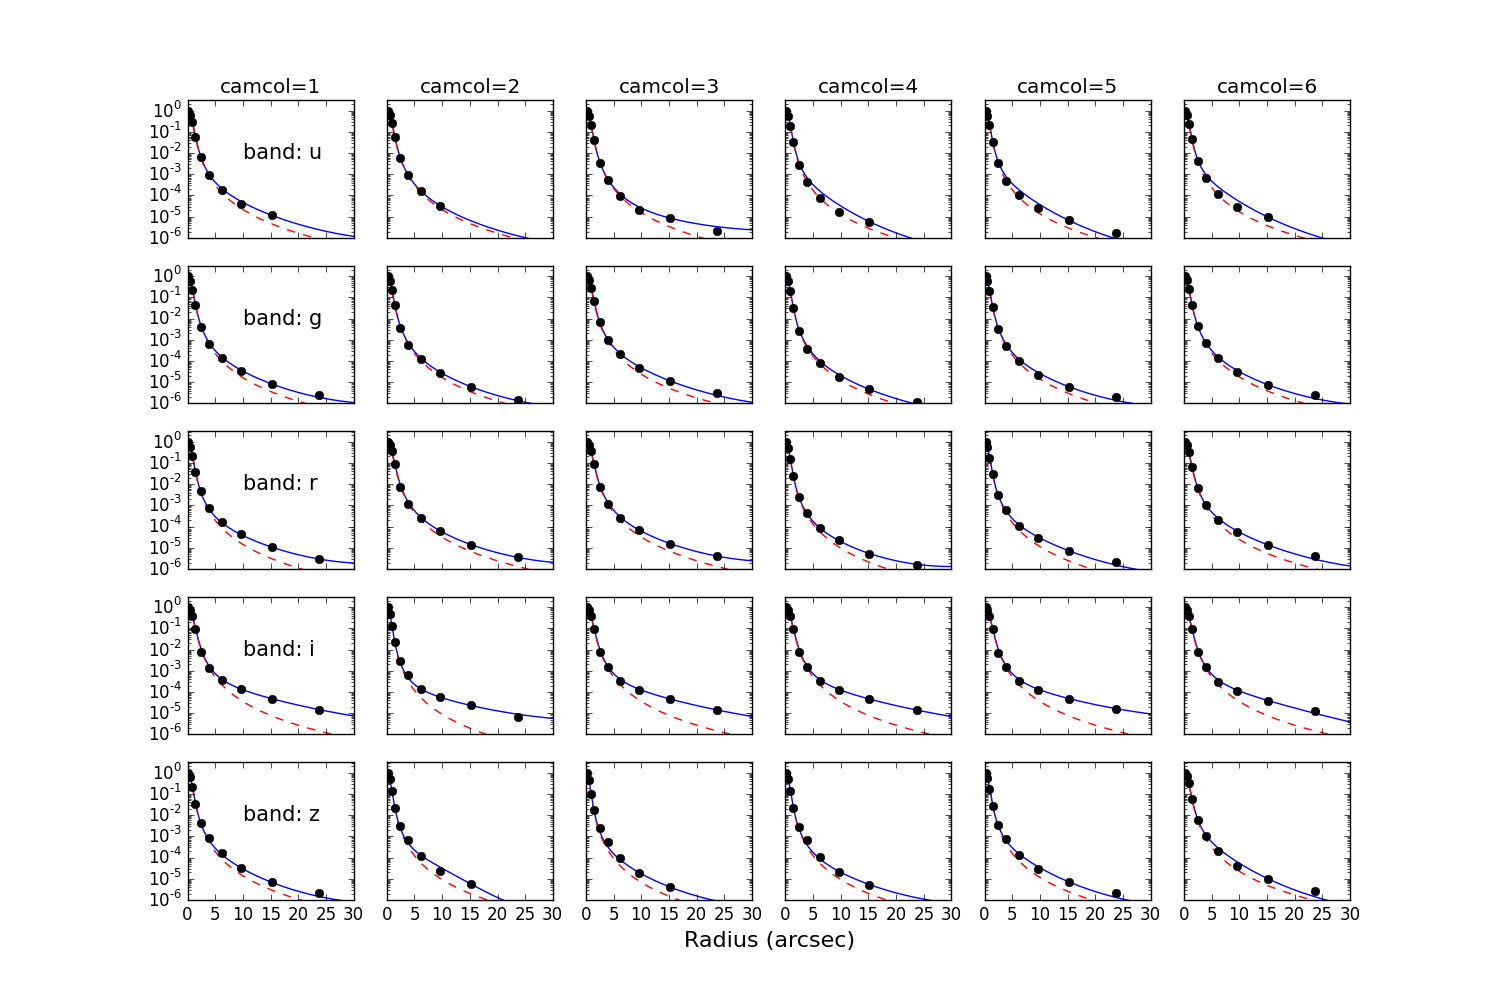
\includegraphics[width=0.9\textwidth]{FIGURES/psffit.png}
\caption{Fit to the PSF profiles from run 4874, field 0. Red curves
  are results of 1-parameter von Karman fits. Blue curves are red
  curve convolved with the instrument PSF, where the scaling factor on
  the tail component is allowed to vary. Note that the y-axis is on
  logorithm scale.
\label{fig:psffit}}
\end{figure}
